\documentclass[a4paper, 12pt]{article}
\usepackage[T2A,T1]{fontenc}
\usepackage[utf8]{inputenc}
\usepackage[english, russian]{babel}
\usepackage{graphicx}
\usepackage[hcentering, bindingoffset = 10mm, right = 15 mm, left = 15 mm, top=20mm, bottom = 20 mm]{geometry}
\usepackage{multirow}
\usepackage{lipsum}
\usepackage{amsmath, amstext}
\usepackage{siunitx}
\usepackage{subcaption}
\usepackage{wrapfig}
\usepackage{adjustbox}
\usepackage{enumerate, indentfirst, float}
\usepackage{capt-of, svg}

\newenvironment{bottompar}{\par\vspace*{\fill}}{\clearpage}
 
\begin{document}
\begin{titlepage}

\newcommand{\HRule}{\rule{\linewidth}{0.5mm}} % Defines a new command for the horizontal lines, change thickness here

\center % Center everything on the page
 
%----------------------------------------------------------------------------------------
%	HEADING SECTIONS
%----------------------------------------------------------------------------------------

\textsc{\LARGE Московский Физико-Технический Институт}\\[1,5cm] % Name of your university/college
\textsc{\Large Кафедра общей физики}\\[0.5cm] % Major heading such as course name
\textsc{\large Лабораторная работа \textnumero  3.3.1}\\[0.5cm] % Minor heading such as course title

%----------------------------------------------------------------------------------------
%	TITLE SECTION
%----------------------------------------------------------------------------------------

\HRule
\\[0.4cm]
{ \huge \bfseries Измерение удельного заряда электрона методами магнитной фокусировки и магнетрона}
\\[0.2cm] % Title of your document
\HRule
\\[1.5cm]


 
%----------------------------------------------------------------------------------------
%	AUTHOR SECTION
%----------------------------------------------------------------------------------------

\begin{minipage}{0.4\textwidth}
	\begin{flushleft} \large
		\emph{Автор:}\\
		Ришат \textsc{Исхаков} % Your name
	\end{flushleft}
\end{minipage}
~
\begin{minipage}{0.4\textwidth}
	\begin{flushright} \large
		\emph{Преподаватель:} \\
		Александр Александрович \textsc{Казимиров} % Supervisor's Name
	\end{flushright}
\end{minipage}

\begin{bottompar}
	\begin{center}
		\includegraphics[width = 80 mm]{logo.jpg}
	\end{center}
	{\large \today}

\end{bottompar}
\vfill % Fill the rest of the page with whitespace

\end{titlepage}

\section{Цель работы}

Определение отношения заряда электрона к его массе двумя методами.

\subsection*{Метод магнитной фокусировки}

В работе используются: \textit{электронно-лучевая трубка и блок питания к ней; источник постоянного тока; соленоид; электростатический вольтметр; милливеберметр; ключи.}\\[0.5cm]
Если поместить электронно-лучевую трубку вынутую из осциллографа в длинный соленоид, который будет создавать магнитное поле, направленное вдоль оси трубки, то электроны, вылетающие из катода, ускоряемые анодным напряжением $V_{\text{уск}}$ , пройдя сквозь две узкие диафрагмы, окажутся с примерно с одинаковыми продольными скоростями. Небольшое напряжение на отклоняющие пластины будет изменять только поперечную составляющую скорости, потому что продольная составляющая параллельна вектору магнитной индукции $\overrightarrow{B}$. Затем постепенно увеличиваем магнитное поле, вследствие чего увеличится сила Лоренца, действующая на электрон и линия будет постепенно стягиваться в точку. Это будет соответствовать положению фокуса. Увеличивая магнитное поле дальше заметим, что электрон будет описывать несколько витков. Используем это для определения удельного заряда электрона.

\subsection*{Метод Магнетрона}

В работе используются: \textit{электронная лампа с цилиндрическим анодом; соленоид; источники питания лампы и соленоида; вольтметр постоянного тока; миллиамперметр.}\\[0.5cm]
В данном эксперименте используется конфигурация магнитного и электрического полей. В соленоид помещается двухэлектродная лампа с цилиндрическим анодом. В качестве катода используется тонкая вольфрамовая проволока. Нить разогревается переменным током от источника питания. На вылетающие электроны действует сила, возникающая в электрическом поле и сила Лоренца. Увеличение магнитного поля приводит к отклонению траектории электрона от прямой. После преодолевания критического значения магнитной индукции электрон перестает долетать до анода и, соответственно, падает анодный ток.

\begin{figure}[H]
\centering
	 \includegraphics[width = 80 mm]{expected.png}
\caption{Ожидаемая зависимость тока от величины магнитной индукции}
\label {img:expected}
\end{figure}



\section{Работа и измерения}
\subsection*{Метод магнитной фокусировки}
Параметры установки: 

$SN = 3000 \: \text{см}^2$

$l = 26,5 \: \text{см}$

Магнитную индукцию будем рассчитывать по формуле:
$$B = \dfrac{\Phi}{SN}$$
\begin{figure}[H]
\parbox[H]{0.3\textwidth}{\null
  \centering
  \includegraphics[width = \linewidth]{focus}
  \captionof{figure}{Схема установки для измерений $e/m$ методом магнитной фокусировки}}
\parbox[H]{0.65 \textwidth}{\null
\centering
  \begin{tabular}{|c|c|c|c|c|}
\hline
$\Phi_1, mWb$  & $\Phi_2, mWb$  & $\Phi_2 - \Phi_1, mWb$  & $I, \text{А}$   & $B, \text{мТ}$   \\ \hline
1.0 & 5.8 & 4.8 & 3.53 & 16.0 \\ \hline
0.7 & 5.6 & 4.9 & 3.65 & 16.3 \\ \hline
1.5 & 5.5 & 4.0 & 2.98 & 13.3 \\ \hline
2.1 & 5.4 & 3.3 & 2.51 & 11.0 \\ \hline
2.7 & 5.3 & 2.6 & 1.90 & 8.7  \\ \hline
2.9 & 5.2 & 2.3 & 1.66 & 7.7  \\ \hline
3.3 & 5.1 & 1.8 & 1.31 & 6.0  \\ \hline
3.6 & 5.0 & 1.4 & 1.02 & 4.7  \\ \hline
4.0 & 4.9 & 0.9 & 0.82 & 3.0  \\ \hline
4.6 & 4.8 & 0.2 & 0.18 & 0.7  \\ \hline
\end{tabular}
\captionof{table}[t]{Полученные значения}%
}
\end{figure}

\begin{figure}[H]
\centering
	 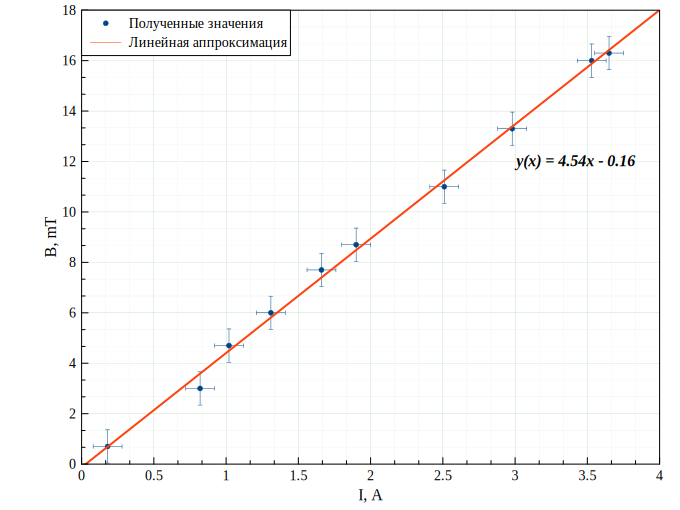
\includegraphics[width = 0.7 \textwidth]{Graph1}
\caption{Зависимость $B = f(I)$ в прямом направлении}
\label {img:b(i)straight}
\end{figure}

\begin{figure}[H]
\centering
	 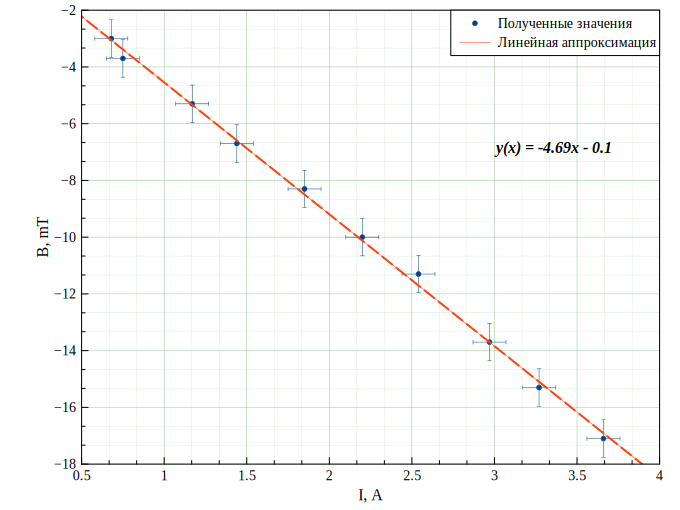
\includegraphics[width = 0.7 \textwidth]{Graph2}
\caption{Зависимость $B = f(I)$ в обратном направлении}
\label {img:b(i)otherwise}
\end{figure}

По полученным уравнениям можно найти уравнение, которое потом используем для нахождения магнитной индукции от произвольного значения тока в цепи:$$B(I) = \dfrac{4.54 + \vert -4.69 \vert}{2}I - \dfrac{0.16 + 0.1}{2} = 4.61I-0.13$$

\begin{table}[H]
\centering
\begin{tabular}{|c|c|c|c|c|c|c|}
\hline
$V_{\text{уск}}, \text{кВ}$                     & Направление        & $I_{\Phi}, \text{А}$   & $n$ & $B, \text{мТ}$     & $\Delta B, \text{мТ}$   & $e/m, 10^{11} \: \text{Кл/кг}$        \\ \hline
\multirow{10}{*}{0.94} & \multirow{5}{*}{1} & 0.59 & 1 & 2.59   & 0.16 & 1.58 \\ \cline{3-7} 
                       &                    & 1.18 & 2 & 5.31   & 0.20 & 1.56 \\ \cline{3-7} 
                       &                    & 1.67 & 3 & 7.57   & 0.25 & 1.55 \\ \cline{3-7} 
                       &                    & 2.40 & 4 & 10.93  & 0.29 & 1.41 \\ \cline{3-7} 
                       &                    & 3.02 & 5 & 13.79  & 0.33 & 1.39 \\ \cline{2-7} 
                       & \multirow{5}{*}{2} & 0.61 & 1 & 2.68  & 0.05 & 1.47 \\ \cline{3-7} 
                       &                    & 1.20 & 2 & 5.40  & 0.09 & 1.45 \\ \cline{3-7} 
                       &                    & 1.81 & 3 & 8.21  & 0.12 & 1.41 \\ \cline{3-7} 
                       &                    & 2.37 & 4 & 10.80 & 0.16 & 1.45 \\ \cline{3-7} 
                       &                    & 2.96 & 5 & 13.52 & 0.19 & 1.45 \\ \hline
\multirow{11}{*}{0.8}  & \multirow{5}{*}{1} & 0.55 & 1 & 2.41  & 0.05 & 1.55 \\ \cline{3-7} 
                       &                    & 1.09 & 2 & 4.89  & 0.08 & 1.50 \\ \cline{3-7} 
                       &                    & 1.67 & 3 & 7.57  & 0.11 & 1.41 \\ \cline{3-7} 
                       &                    & 2.21 & 4 & 10.06 & 0.15 & 1.42 \\ \cline{3-7} 
                       &                    & 2.70 & 5 & 12.32 & 0.18 & 1.48 \\ \cline{2-7} 
                       & \multirow{6}{*}{2} & 0.54 & 1 & 2.36   & 0.16 & 1.62 \\ \cline{3-7} 
                       &                    & 1.10 & 2 & 4.94   & 0.20 & 1.47 \\ \cline{3-7} 
                       &                    & 1.70 & 3 & 7.71   & 0.24 & 1.36 \\ \cline{3-7} 
                       &                    & 2.27 & 4 & 10.33  & 0.28 & 1.35 \\ \cline{3-7} 
                       &                    & 2.79 & 5 & 12.73  & 0.32 & 1.39 \\ \cline{3-7} 
                       &                    & 3.39 & 6 & 15.50  & 0.36 & 1.35 \\ \hline
\end{tabular}
\caption{Данные измерения зависимости номера фокуса от тока}
\end{table}

Используя формулу найдем значение удельного заряда: 
$$\dfrac{e}{m} = \dfrac{8\pi^2Vn^2}{l^2B_\text{ф}^2}$$
Полученное значение удельного заряда:
$\dfrac{e}{m} = (1.55 \pm 0.4 )\cdot 10^{11}  \: \text{Кл/кг}$


\section{Метод магнетрона}


\begin{wrapfigure}[11]{l}{5.2cm}
\includegraphics[width=5.5cm]{magnetron}
\caption{Схема установки}
\end{wrapfigure} 

		Параметры установки: $$k = 0.035 \:\text{Т/А}$$
$$r_a = 12 \:\text{мм}$$
Для разных потенциалов $V$ на анодной лампе снимем зависимость анодного тока $I_a$ от тока $I_\text{m}$ через соленоид. По коэффициенту установки найдем значение магнитной индукции в зависимости от тока через соленоид: $B = kI_m$
\vspace{4 cm}
\begin{table}[H]
\centering
\caption{$V = 70 \: \text{В}$}
\begin{adjustbox}{max width=\textwidth}
\begin{tabular}{|c|c|c|c|c|c|c|c|c|c|c|c|c|c|c|c|c|c|c|c|c|c|c|}
\hline
$I_a, \text{мА}$ & 0.23 & 0.23 & 0.23 & 0.23 & 0.22 & 0.22 & 0.19 & 0.10 & 0.02 & 0.01 & 0.08 & 0.22 & 0.22 & 0.20 & 0.16 & 0.12 & 0.10 & 0.18 & 0.01 & 0.09 & 0.06 & 0.04 \\ \hline
$I_m, \text{А}$  & 0.10 & 0.06 & 0.05 & 0.09 & 0.12 & 0.12 & 0.12 & 0.13 & 0.13 & 0.14 & 0.13 & 0.10 & 0.11 & 0.12 & 0.13 & 0.13 & 0.13 & 0.13 & 0.14 & 0.13 & 0.13 & 0.13 \\ \hline
$B,\text{мТ}$    & 3.5  & 2.1  & 1.68 & 3.08 & 4.2  & 4.2  & 4.34 & 4.48 & 4.55 & 4.76 & 4.48 & 3.36 & 3.78 & 4.34 & 4.41 & 4.48 & 4.48 & 4.41 & 4.83 & 4.48 & 4.48 & 4.48 \\ \hline
\end{tabular}
\end{adjustbox}
\end{table}

\begin{figure}[H]
\centering
	 \includegraphics[width = 0.6 \textwidth]{Figure3}
\caption{Зависимость $B = f(I_a)$ для $V = 70 \: \text{В}$}
\end{figure}

\begin{table}[H]
\centering
\caption{$V = 80 \: \text{В}$}
\begin{adjustbox}{max width=\textwidth}
\begin{tabular}{|c|c|c|c|c|c|c|c|c|c|c|c|c|c|c|c|c|c|c|}
\hline
$I_a, \text{мА}$ & 0.24 & 0.24 & 0.24 & 0.23 & 0.23 & 0.23 & 0.23 & 0.07 & 0.22 & 0.20 & 0.14 & 0.06 & 0.04 & 0.03 & 0.02 & 0.01 & 0.01 & 0.12 \\ \hline
$I_m, \text{А}$  & 0.00 & 0.02 & 0.04 & 0.06 & 0.08 & 0.10 & 0.12 & 0.13 & 0.13 & 0.13 & 0.13 & 0.13 & 0.14 & 0.14 & 0.14 & 0.14 & 0.14 & 0.13 \\ \hline
$B, \text{мТ}$    & 0.0  & 0.7  & 1.4  & 2.1  & 2.8  & 3.5  & 4.2  & 4.69 & 4.62 & 4.62 & 4.62 & 4.69 & 4.76 & 4.76 & 4.83 & 4.9  & 5.04 & 4.62 \\ \hline
\end{tabular}
\end{adjustbox}
\end{table}

\begin{figure}[H]
\centering
	 \includegraphics[width = 0.6 \textwidth]{80V}
\caption{Зависимость $B = f(I_a)$ для $V = 80\: \text{В}$}
\end{figure}

\begin{table}[H]
\centering
\caption{$V = 90 \: \text{В}$}
\begin{adjustbox}{max width=\textwidth}
\begin{tabular}{|c|c|c|c|c|c|c|c|c|c|c|c|c|c|c|c|c|c|c|}
\hline
$I_a, \text{мА}$ & 0,23 & 0,24 & 0,24 & 0,24 & 0,24 & 0,24 & 0,24 & 0,22 & 0,20 & 0,17 & 0,14 & 0,10 & 0,07 & 0,05 & 0,03 & 0,02 & 0,01 & 0,01 \\ \hline
$I_m, \text{А}$  & 0,00 & 0,02 & 0,04 & 0,06 & 0,08 & 0,10 & 0,12 & 0,14 & 0,14 & 0,14 & 0,14 & 0,14 & 0,14 & 0,15 & 0,15 & 0,15 & 0,15 & 0,16 \\ \hline
$B,\text{мТ}$    & 0    & 0,7  & 1,4  & 2,1  & 2,8  & 3,5  & 4,2  & 4,9  & 4,97 & 4,97 & 5,04 & 5,04 & 5,04 & 5,11 & 5,11 & 5,18 & 5,32 & 5,46 \\ \hline
\end{tabular}
\end{adjustbox}
\end{table}

\begin{figure}[H]
\centering
	 \includegraphics[width = 0.6 \textwidth]{90V}
\caption{Зависимость $B = f(I_a)$ для $V = 90\: \text{В}$}
\end{figure}

\begin{table}[H]
\centering
\caption{$V = 100 \:\text{В}$}
 \begin{adjustbox}{max width=\textwidth}
\begin{tabular}{|c|c|c|c|c|c|c|c|c|c|c|c|c|c|c|c|c|c|c|}
\hline
$I_a, \text{мА}$ & 0.24 & 0.24 & 0.24 & 0.24 & 0.24 & 0.24 & 0.24 & 0.23 & 0.22 & 0.20 & 0.16 & 0.14 & 0.10 & 0.08 & 0.05 & 0.03 & 0.02 & 0.01 \\ \hline
$I_m, \text{А}$  &0.00 & 0.02 & 0.04 & 0.06 & 0.08 & 0.10 & 0.12 & 0.14 & 0.15 & 0.15 & 0.15 & 0.15 & 0.15 & 0.15 & 0.15 & 0.16 & 0.16 & 0.16 \\ \hline
$B,\text{мТ}$& 0    & 0.7  & 1.4  & 2.1  & 2.8  & 3.5  & 4.2  & 4.9  & 5.18 & 5.25 & 5.25 & 5.25 & 5.32 & 5.32 & 5.32 & 5.46 & 5.6  & 5.74 \\ \hline
\end{tabular}
\end{adjustbox}
\end{table}

\begin{figure}[H]
\centering
	 \includegraphics[width = 0.6 \textwidth]{100V}
\caption{Зависимость $B = f(I_a)$ для $V = 100\: \text{В}$}
\end{figure}

\begin{table}[H]
\centering
\caption{$V = 110 \: \text{В}$}
 \begin{adjustbox}{max width=\textwidth}
\begin{tabular}{|c|c|c|c|c|c|c|c|c|c|c|c|c|c|c|c|c|c|c|c|c|}
\hline
$I_a, \text{мА}$ & 0,24 & 0,24 & 0,24 & 0,24 & 0,24 & 0,24 & 0,24 & 0,23 & 0,23 & 0,19 & 0,16 & 0,13 & 0,05 & 0,11 & 0,07 & 0,04 & 0,03 & 0,02 & 0,01 & 0,01 \\ \hline
$I_m, \text{А}$  & 0,00 & 0,02 & 0,04 & 0,06 & 0,08 & 0,10 & 0,12 & 0,14 & 0,15 & 0,16 & 0,16 & 0,16 & 0,16 & 0,16 & 0,16 & 0,16 & 0,16 & 0,17 & 0,17 & 0,18 \\ \hline
$B,\text{мТ}$ & 0    & 0,7  & 1,4  & 2,1  & 2,8  & 3,5  & 4,2  & 4,9  & 5,32 & 5,46 & 5,53 & 5,53 & 5,6  & 5,6  & 5,6  & 5,67 & 5,74 & 5,88 & 6,02 & 6,16 \\ \hline
\end{tabular}
\end{adjustbox}
\end{table}

\begin{figure}[H]
\centering
	 \includegraphics[width = 0.6 \textwidth]{110V}
\caption{Зависимость $B = f(I_a)$ для $V = 110\: \text{В}$}
\end{figure}

\begin{table}[H]
\centering
\caption{$V = 120\:  \text{В}$}
 \begin{adjustbox}{max width=\textwidth}
\begin{tabular}{|c|c|c|c|c|c|c|c|c|c|c|c|c|c|c|c|c|c|c|c|c|c|}
\hline
$I_a,\text{мА}$ & 0,24 & 0,24 & 0,24 & 0,24 & 0,24 & 0,24 & 0,24 & 0,24 & 0,23 & 0,21 & 0,17 & 0,15 & 0,13 & 0,11 & 0,09 & 0,07 & 0,05 & 0,03 & 0,02 & 0,01 & 0,01 \\ \hline
$I_m,\text{А}$  & 0,00 & 0,02 & 0,04 & 0,06 & 0,08 & 0,10 & 0,12 & 0,14 & 0,16 & 0,16 & 0,17 & 0,17 & 0,17 & 0,17 & 0,17 & 0,17 & 0,17 & 0,17 & 0,18 & 0,18 & 0,18 \\ \hline
$B,\text{мТ}$  & 0    & 0,7  & 1,4  & 2,1  & 2,8  & 3,5  & 4,2  & 4,9  & 5,6  & 5,74 & 5,81 & 5,81 & 5,88 & 5,88 & 5,88 & 5,88 & 5,95 & 6,02 & 6,16 & 6,3  & 6,44 \\ \hline
\end{tabular}
\end{adjustbox}
\end{table}

\begin{figure}[H]
\centering
	 \includegraphics[width = 0.6 \textwidth]{120V}
\caption{Зависимость $B = f(I_a)$ для $V = 120\: \text{В}$}
\end{figure}

По графикам определим значение $B_\text{кр}$ и построим таблицу:

\begin{table}[H]
\centering
\begin{tabular}{|c|c|c|c|}
\hline
$B_{\text{кр}}$, мТ & $V$, B & $B_{\text{кр}}^2, \text{(мТ)}^2$ & $\Delta B_{\text{кр}}^2, \text{(мТ)}^2$ \\ \hline
4,5     & 70   & 20,07       & 0,90         \\ \hline
4,7     & 80   & 21,62       & 0,93         \\ \hline
5,1     & 90   & 25,50       & 1,01         \\ \hline
5,3     & 100  & 28,09       & 1,06         \\ \hline
5,6     & 110  & 30,80       & 1,11         \\ \hline
5,9     & 120  & 34,81       & 1,18         \\ \hline
\end{tabular}
\end{table}

\begin{figure}[H]
\centering
	 \includegraphics[width = 0.7 \textwidth]{Graph3}
\caption{Зависимость $B_{\text{кр}}^2$ от $V$}
\end{figure}

Тогда по формуле найдем удельный заряд электрона в данном методе $$\dfrac{e}{m} = \dfrac{8V}{B_{\text{кр}}r_a^2} = (1.87 \pm 0.17) \cdot 10^{11} \: \text{Кл/кг}$$

\section{Вывод}

Полученное двумя способами значение удельного заряда электрона с учетом погрешности соответствует действительности. 

В первом эксперименте основную погрешность измерения составляет ошибка, связанная с калибровкой электромагнита: имеется внешнее магнитное поле, которое нельзя считать постоянным и поэтому невозможно полностью избавиться от него в конечном результате с помощью полусуммы. Еще больший вклад в ошибку добавляет невозможность полностью определить момент, при котором линия полностью стягивается в точку. При значениях порядкового номера фокуса $\geq 3$ становится сложно определить точный момент.

Во втором эксперименте погрешность измерения меньше, так как исключается влияние внешних факторов. Основная погрешность обусловлена достаточно старыми приборами, в которых перемещение стрелки при маленьких изменениях ограничивается силой трения.

\end{document}